% 行为学结果
% - [ ] 小鼠行为学结果
%   - [ ] 行为范式说明
% - [ ] 患者行为学结果
%   - [ ] 行为范式说明
%   - [ ] 韦伯定律
%   - [ ] 行为分布图
%   - [ ] 行为学提示所需的任务可能与增强学习相关

\section{小鼠的时间间隔预测行为}
为了探究视觉信息对小鼠的时间感知的影响,尤其是对视觉刺激所编码的时间的感知,
我们设计了连续周期性视觉刺激时间预测行为实验。通过耦连视觉刺激与小鼠舔水行为,
我们可以检测小鼠的舔水来推断小鼠内在的计时。

\subsection{规律刺激下的小鼠时间预测行为}
% 行为学范式示意图
% 一天舔水的示例
% 第一次舔水的分布曲线
% weber定律
我们选用了经过限水处理的野生型C57小鼠作为实验对象,每天包含5次连续的训练,
每次训练包含20个规律性的刺激。每次视觉刺激持续1秒,刺激间间隔为9秒;
每次刺激开始时小鼠均可以获得一定的水作为正向的反馈(图\ref{fig:mouse_behavior})。

为了评判小鼠在一天中的行为表现,我们将一天中小鼠舔水的行为时刻做了记录;
并以每次视觉刺激的开始作为原点,将前8秒和后2秒作为事件窗口对舔水行为做了分组。
同时,我们将不同组的行为以第一次舔水的时刻点做了排序(图\ref{fig:mouse_behavior})。
为了进一步比较不同天之间小鼠的行为表现,我们将第一次舔水的时刻点单独拿出来,
并对在视觉刺激之前发生的行为做了累计分布曲线(图\ref{fig:mouse_behavior})。
我们可以看到随着训练天数的增加,小鼠的舔水时刻向刺激开始的时间靠近。
前三天和后三天舔水的平均分布之间也存在统计学上的显著差异
(Kolmogorov–Smirnov检验,p值为$2.3 \times 10 ^ {-41}$), 提示了
小鼠在训练过程中存在着学习过程, 对刺激间时间间隔的感知准确度有所提高。

另一方面,我们也通过计算了小鼠行为学的韦伯系数(weber's fraction)
来检验小鼠对时间间隔的感知精确度(图\ref{fig:mouse_behavior})。
由于时间所限,我们未能对大量的老鼠
来做行为学;但我们依然能够看到随着训练时间的延长,小鼠行为学的韦伯系数
呈下降趋势。

综合小鼠的行为学结果来看,我们可以推断在连续周期性视觉刺激时间预测行为实验中,
小鼠对刺激间时间间隔的感知的精确度和准确度均有一定的提升,提示小鼠可能存在
学习过程;而小鼠大脑中神经元之间是否有发生动态的变化,还需要进一步的电生理实验
来验证。

\begin{figure}[h]
    \begin{center}
    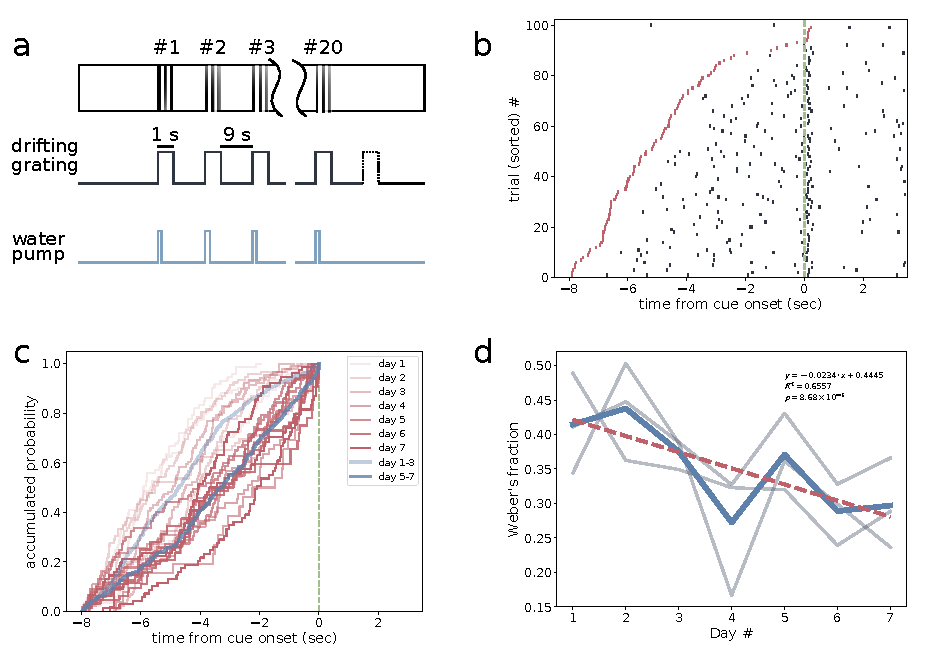
\includegraphics[width=\textwidth]{src/figures/mouse_behavior.pdf}
    \end{center}

    \caption{\textbf{规律刺激下的小鼠时间预测行为}\\
    一些额外的图注说明}
    \label{fig:mouse_behavior}
\end{figure}

%%%%%%%%%%%%%%%%%%%%%%%%%%%%%%%%%%%%%%%%%%%%%%%%%%%%%%%%%%%%%%%%
\section{患者的时间间隔预测行为}
为了进一步探究人脑对时间间隔的感知,我们对小鼠的行为学范式稍加改进后用于
对人的实验。对于相同类型的视觉刺激,我们设计了不同的时间间隔,包括4秒和9秒间隔;
以及不同的行为范式,包括轻拍手,默想和空想(图\ref{fig:human_behavior}~a)。
轻拍手下被试需要主动判断预测的同时,还需要行为上的输出;
在默想范式下,则只需要主动判断预测;
而空想范式中更多的只是体现单纯的视觉刺激造成的影响。

同时,我们选择了没有患癫痫的正常人进行了行为学实验,以作为对照组进行参考。

\subsection{韦伯定律}
我们首先计算了不同天里的行为学韦伯系数(图\ref{fig:human_behavior}~b),
并对5秒间隔和10秒间隔进行了对比,结果两者之间没有统计学上的显著性差异
(t检验,t统计量为1.130,p值为0.259)。表明两种间隔的行为没有差别,与
韦伯定律相符合\cite{gibbon1977scalar, hardy2018encoding}。

同时,我们计算了韦伯系数的线性相关系数,但没有统计学上的显著性(t检验, p值分别为0.570和0.417);
提示患者在不同天里的行为学表现没有显著的变化,可能是因为每天进行行为学实验的时间
并不是很长(约30分钟),并不足以形成稳定的记忆。因此,我们可以将不同天的行为学认为
是在同一天内进行的。

为了进一步评估一天内行为学表现可能的变化,我们将每天的20次刺激分为5份(quintiles),
分别计算每份的韦伯系数(图\ref{fig:human_behavior}~c)。
但5秒间隔,10秒间隔和对照组的5份间的韦伯系数没有统计学上的显著性差异
(one-way ANOVA, F统计量分别为3.309, 0.841和0.019,p值为0.057,0.497和0.996)。
但可以看到第一份的韦伯系数较后四份的有更大的趋势;同时考虑到实验中,患者自我调整
的速度很快。这一现象可能是由于患者在第一份的中间就已经很好的把握了时间间隔,
并能够较为准确的预测了。
而在过去类似的行为学范式中,也同样存在类似的快速学习的过程\cite{simen2011model}。

\subsection{轻拍手行为分布}
由于将行为学表现抽象为

\subsection{行为结果所体现的可能的理论机制}

\begin{figure}[h]
    \centering
    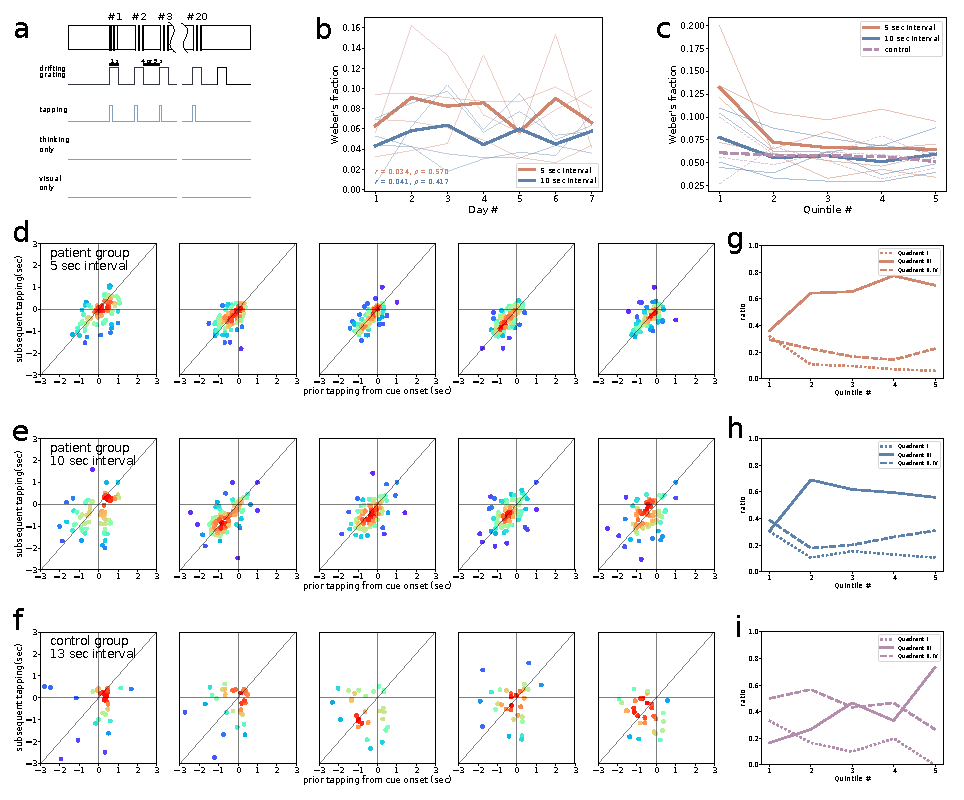
\includegraphics[width=\textwidth]{src/figures/human_behavior.pdf}
    \caption{规律刺激下的人的时间预测行为}
    \label{fig:human_behavior}
\end{figure}





